\section{应用正交设计}
\label{sec:apply-orthogonal-design}

\begin{frame}
  \begin{center}
    \Huge{\textcolor{red}{应用正交设计}}
  \end{center}
\end{frame}

\subsection{迭代1}

\begin{frame}[fragile]{需求1:在仓库中查找所有颜色为红色的产品}
  \begin{java}
public static ArrayList findAllRedProducts(ArrayList repo) {
  ArrayList result = new ArrayList();
  for (int i=0; i<repo.size(); i++) {
    Product product = (Product)repo[i];
    if (product.getColor() == Color.RED) {
       result.add(product);
    }
  }
  return result;
}
  \end{java}
\end{frame}

\begin{frame}[fragile]{识别坏味道}
\begin{enumerate}
  \item 缺乏编译时类型安全性检查
  \item 依赖于具体实现类型
  \item 硬编码  
  \item 传递容器
\end{enumerate}
\end{frame}

\begin{frame}[fragile]{简单重构}
  \begin{java}
public static List<Product> findAllRedProducts(
  List<Product> repo) {
  List<Product> result = new ArrayList<>();
  for (Product p : repo) {
    if (p.getColor() == Color.RED) {
      result.add(p);
    }
  }
  return result;
}
  \end{java}

\begin{enumerate}
  \item 引入泛型,增强编译时类型安全
  \item 依赖于更加抽象的List,而非具体的ArrayList
  \item 使用foreach迭代,避免错误发生的风险
\end{enumerate}  
\end{frame}

\subsection{迭代2}

\begin{frame}[fragile]{需求2:在仓库中查找所有颜色为绿色的产品}
  \begin{java}
public static List<Product> findAllGreenProducts(
  List<Product> repo) {
  List<Product> result = new ArrayList<>();
  for (Product p : repo) {
    if (p.getColor() == Color.GREEN) {
      result.add(p);
    }
  }
  return result;
}
  \end{java}

\begin{enumerate}
  \item 复制/粘贴:导致重复设计
  \item 策略:消除重复
\end{enumerate}  
\end{frame}

\begin{frame}[fragile]{消除重复:参数化}
  \begin{java}
public static List<Product> findProductsByColor(
  List<Product> repo, Color color) {
  List<Product> result = new ArrayList<>();
  for (Product p : repo) {
    if (p.getColor() == color) {
      result.add(p);
    }
  }
  return result;
}
  \end{java}

\begin{enumerate}
  \item 参数化设计,是最常用,最简单的消除重复的手段
\end{enumerate}  
\end{frame}

\subsection{迭代3}

\begin{frame}[fragile]{需求3:查找所有重量小于10的所有产品}
  \begin{java}
public static List<Product> findProductsBelowWeight(
  List<Product> repo, int weight) {
  List<Product> result = new ArrayList<>();
  for (Product p : repo) {
    if (p.getWeight() < weight) {
      result.add(p);
    }
  }
  return result;
}
  \end{java}

\begin{enumerate}
  \item 两个参数化实现:重复再现
\end{enumerate}  
\end{frame}

\begin{frame}[fragile]{消除重复:糟糕的设计}
  \begin{java}
public List<Product> findProducts(
  List<Product> repo, Color color, int weight, boolean flag) {
  List<Product> result = new ArrayList<>();
  for (Product p : repo) {
    if ((flag && p.getColor() == color) ||
       (!flag && p.getWeight() < weight)) {
      result.add(p);
    }
  }
  return result;
}
  \end{java}  

\begin{enumerate}
  \item 如果强制再次使用参数化消除两者之间的重复,必然增加设计的复杂度,得不偿失
  \item 参数化设计抽象能力较弱,意味着缺失更加稳定的抽象  
\end{enumerate}    
\end{frame}

\subsection{提取抽象}

\begin{frame}[fragile]{提取抽象}
  \begin{java}
public interface ProductSpec {
  boolean satisfy(Product product);
}
  \end{java}

\begin{enumerate}
  \item 愚弄我一次,应感到羞愧的是你;再次愚弄我,应该羞愧的是我。
  \item 愿意被第一颗子弹击中,确保不再被同一支枪发射的同个方向发射的子弹。
  \item 0, 1, N
\end{enumerate}
\end{frame}

\begin{frame}[fragile]{分离关注点:职责单一,开放封闭}
  \begin{java}
public static List<Product> findProducts(
  List<Product> repo, ProductSpec spec) {
  List<Product> result = new ArrayList<>();
  for (Product p : repo) {
    if (spec.satisfy(p)) {
      result.add(p);
    }
  }
  return result;
}
  \end{java}
\begin{enumerate}
  \item 集合类型: List<Product>
  \item 迭代算法: 线性算法
  \item 匹配规则: ProductSpec
\end{enumerate}    
\end{frame}

\begin{frame}[fragile]{算子:封装变化1}
  \begin{java}
public class ColorSpec implements ProductSpec {
  private Color color;

  public ColorSpec(Color color) {
    this.color = color;
  }

  @Override
  public boolean satisfy(Product product) {
    return product.getColor() == color;
  }
}
  \end{java}

\begin{enumerate}
  \item 算法实现模块与该具体匹配规则,通过更抽象的ProductSpec实现解耦
\end{enumerate}      
\end{frame}


\begin{frame}[fragile]{算子:封装变化2}
  \begin{java}
public class BelowWeightSpec implements ProductSpec {
  private int limit;

  public BelowWeightSpec(int limit) {
    this.limit = limit;
  }

  @Override
  public boolean satisfy(Product product) {
    return product.getWeight() < limit;
  }
}
  \end{java}

\begin{enumerate}
  \item 坏味道:两个算子显现结构性重复
\end{enumerate}        
\end{frame}

\begin{frame}[fragile]{重构到模式}
  \begin{figure}
    \centering
    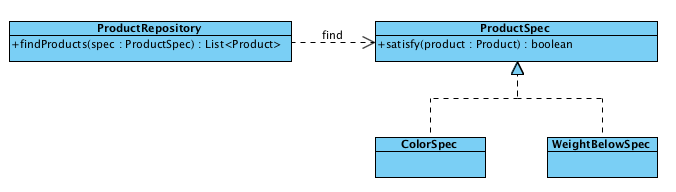
\includegraphics[width=1.0\textwidth]{strategy-pattern.png}
  \end{figure}
\begin{enumerate}
  \item 设计模式引入,是遵循良好的设计原则的自然结果
  \item 不恰当的滥用或误用,必然会增加设计的复杂度
\end{enumerate}        

\end{frame}

\subsection{封装}

\begin{frame}[fragile]{封装}
  \begin{java}
public class ProductRepository {
  private List<Product> products = new ArrayList<>();

  public void add(Product p) {
    products.add(p);
  }

  public List<Product> findProducts(ProductSpec spec) {
    List<Product> result = new ArrayList<>();
    for (Product p : products) {
      if (spec.satisfy(p)) {
        result.add(p);
      }
    }
    return result;
  }
}
  \end{java}

\begin{enumerate}
  \item 封装: 将具体实现的数据结构封装起来,并将其算法实现搬迁至领域对象
  \item 警惕缺乏封装的static方法,常常违背了良好的OO设计原则  
\end{enumerate}          
\end{frame}

\begin{frame}[fragile]{存储:客户相关}
  \begin{java}
public class ProductDb {
  private Database db = new Database();
  private ProductRepository repo;

  public ProductDb(ProductRepository repo) {
    this.repo = repo;
  }

  public void save() {
    for (Product p : repo.getAllProducts()) {
      db.save(p);
    }
  }
}
  \end{java}

  \begin{enumerate}
    \item 该业务算法实现,导致repo.getAllProducts接口的公开,再次开启了传递容器的可能
    \item 搬迁该业务的算法实现至仓库可能不合理,甚至不可行,因为算法实现与该业务实现更加紧密
    \item 如果强行搬迁,也会导致仓库实现的急剧膨胀,并增加两者之间的耦合度
    \item          
  \end{enumerate}
\end{frame}

\begin{frame}[fragile]{更稳定的抽象}
  \begin{java}
@FunctionalInterface
public interface ProductConsumer {
  void accept(Product p);
}
  \end{java}

\begin{enumerate}
  \item 实现仓库与其业务(客户)之间的解耦
\end{enumerate}
\end{frame}

\begin{frame}[fragile]{迭代器}
  \begin{java}
public class ProductRepository {
  private List<Product> products = new ArrayList<>();

  public void add(Product p) {
    products.add(p);
  }

  public void foreach(ProductConsumer consumer) {
    for (Product p : products) {
      consumer.accept(p);
    }
  }
  \end{java}

\begin{enumerate}
  \item 而将仓库内部具体实现的数据结构,及其迭代算法封装起来,实现信息隐藏
\end{enumerate}    
\end{frame}

\begin{frame}[fragile]{常用算法}
  \begin{java}
public class ProductRepository {  
  ...

  public List<Product> findProducts(ProductSpec spec) {
    List<Product> result = new ArrayList<>();
    foreach(p -> {
      if (spec.satisfy(p))
        result.add(p);
    });
    return result;
  }  
}
  \end{java}


\begin{enumerate}
  \item 习惯上,可以将更通用,与业务无关的算法搬迁至仓库;而将其他业务算法实现留在客户本地实现解耦
\end{enumerate}
\end{frame}

\begin{frame}[fragile]{存储:客户相关}
  \begin{java}
public class ProductDb {
  private Database db = new Database();
  private ProductRepository repo;

  public ProductDb(ProductRepository repo) {
    this.repo = repo;
  }

  public void save() {
    repo.foreach(Database::save);
  }
}
  \end{java}

\begin{enumerate}
  \item 例如,数据库相关业务逻辑,留在本地实现将更为恰当;如果搬迁至仓库,会加剧其实现的规模,甚至造成巨类的坏味道,并增加两者之间的耦合度
\end{enumerate}
\end{frame}

\subsection{迭代4}

\begin{frame}[fragile]{需求4:查找所有颜色为红色或者绿色,并且重量小于10的产品}
  \begin{java}
public class ColorAndBelowWeightSpec implements ProductSpec {
  private Color color1; private Color color2;
  private int limit;

  public ColorAndBelowWeightSpec(Color c1, Color c2, int limit) {
    this.color1 = c1; this.color2 = c2;
    this.limit = limit;
  }

  @Override
  public boolean satisfy(Product p) {
    return (p.getColor() == color1 || p.getColor() == color2) 
        && (p.getWeight() < limit);
  }
}
  \end{java}

\begin{enumerate}
  \item 已存在ColorSpec, BelowWeightSpec实现;实现未能更好地复用既有组件,从而导致重复设计
\end{enumerate}  
\end{frame}

\begin{frame}[fragile]{分离关注点:And}
  \begin{java}
public class AndSpec implements ProductSpec {
  private ProductSpec[] specs;

  public AndSpec(ProductSpec... specs) {
    this.specs = specs;
  }

  @Override
  public boolean satisfy(Product p) {
    for (ProductSpec spec : specs) {
      if (!spec.satisfy(p))
        return false;
    }
    return true;
  }
}
  \end{java}
\end{frame}

\begin{frame}[fragile]{分离关注点:Or}
  \begin{java}
public class OrSpec implements ProductSpec {
  private ProductSpec[] specs;

  public OrSpec(ProductSpec... specs) {
    this.specs = specs;
  }

  @Override
  public boolean satisfy(Product p) {
    for (ProductSpec spec : specs) {
      if (spec.satisfy(p))
        return true;
    }
    return false;
  }
}
  \end{java}
\end{frame}

\begin{frame}[fragile]{组合}
  \begin{java}
repo.findProducts(
  new AndSpec(
    new OrSpec(new ColorSpec(RED), new ColorSpec(Greeen)), 
    new BelowWeightSpec(10))
);
  \end{java}

\begin{enumerate}
  \item AndSpec, OrSpec存在重复设计
  \item 客户使用时,承担无聊的new表达式  
\end{enumerate}    
\end{frame}

\begin{frame}[fragile]{消除重复:提取基类}
  \begin{java}
class CombinableSpec implements ProductSpec {
  private ProductSpec[] specs;
  private boolean shortcut;

  protected CombinableSpec(
    ProductSpec[] specs, boolean shortcut) {
    this.specs = specs;
    this.shortcut = shortcut;
  }

  @Override
  public boolean satisfy(Product p) {
    for (ProductSpec spec : specs) {
      if (spec.satisfy(p) == shortcut)
        return shortcut;
    }
    return !shortcut;
  }
}
  \end{java}
\end{frame}

\begin{frame}[fragile]{子类化:配置差异}
  \begin{java}
public class AndSpec extends CombinableSpec {
  public AndSpec(ProductSpec... specs) {
    super(Arrays.asList(specs), false);
  }
}

public class OrSpec extends CombinableSpec {
  public OrSpec(ProductSpec... specs) {
    super(Arrays.asList(specs), true);
  }
}
  \end{java}

\begin{enumerate}
  \item 提取基类后,消除了AndSpec, OrSpec的重复实现
  \item 但是,两者依然存在结构性重复,有待进一步消除
\end{enumerate}   
\end{frame}

\subsection{迭代5}

\begin{frame}[fragile]{需求5:查找所有颜色为不是红色的产品}
  \begin{java}
public class NotSpec implements ProductSpec {
  private ProductSpec spec;

  public NotSpec(ProductSpec spec) {
    this.spec = spec;
  }

  @Override
  public boolean satisfy(Product p) {
    return !spec.satisfy(p);
  }
}

repo.findProducts(
  new NotSpec(new ColorSpec(RED))
);
  \end{java}
\end{frame}

\begin{frame}[fragile]{修饰器}
  \begin{figure}
    \centering
    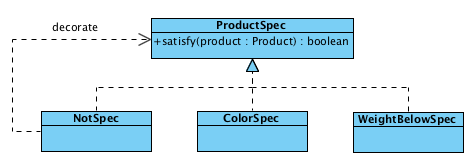
\includegraphics[width=0.95\textwidth]{repo-decorator.png}
  \end{figure}
\end{frame}

\subsection{引入工厂}

\begin{frame}[fragile]{引入工厂}
  \begin{java}
public final class ProductSpecs {
  public static ProductSpec color(Color color) {
    return new ProductSpec() {
      @Override
      public boolean satisfy(Product p) {
        return p.getColor() == color;
      }
    };
  }

  public static ProductSpec not(ProductSpec spec) {
    return new ProductSpec() {
      @Override
      public boolean satisfy(Product p) {
        return !spec.satisfy(p);
      }
    };
  }
}
  \end{java}
\end{frame}

\begin{frame}[fragile]{改善表达力}
  \begin{java}
repo.findProducts(
  new AndSpec(
    new OrSpec(new ColorSpec(RED), new ColorSpec(Greeen)), 
    new BelowWeightSpec(10)
  )
);

repo.findProducts(
  and(
    or(color(RED), color(Greeen)), 
    belowWeight(10)
  )
);
  \end{java}
\end{frame}

\subsection{搬迁工厂方法}

\begin{frame}[fragile]{删除ProductSpecs: Java8}
  \begin{java}
public interface ProductSpec {
  boolean satisfy(Product p);

  static ProductSpec color(Color color) {
    return new ProductSpec() {
      @Override
      public boolean satisfy(Product p) {
        return p.getColor() == color;
      }
    };
  }

  static ProductSpec not(ProductSpec spec) {
    return new ProductSpec() {
      @Override
      public boolean satisfy(Product p) {
        return !spec.satisfy(p);
      }
    };
  }
}
  \end{java}
\end{frame}

\subsection{函数式}

\begin{frame}[fragile]{使用Lambda}
  \begin{java}
findProducts(repo, (Product p) -> p.getColor() == RED);
  \end{java}
\end{frame}

\begin{frame}[fragile]{类型推演}
  \begin{java}
findProducts(repo, p -> p.getColor() == RED);
  \end{java}
\end{frame}

\begin{frame}[fragile]{重构到函数式}
  \begin{java}
@FunctionalInterface
public interface ProductSpec {
  boolean satisfy(Product p);

  static ProductSpec color(Color color) {
    return p -> p.getColor() == color;
  }

  static ProductSpec not(ProductSpec spec) {
    return p -> !spec.satisfy(p);
  }

  ...
}
  \end{java}
\end{frame}

\begin{frame}[fragile]{链式法则: 实现and/or的中缀表达式}
  \begin{java}
@FunctionalInterface
public interface ProductSpec {
  boolean satisfy(Product p);

  static ProductSpec color(Color color) {
    return p -> p.getColor() == color;
  }

  default ProductSpec and(ProductSpec other) {
    return (p) -> satisfy(p) && other.satisfy(p);
  }

  default ProductSpec or(ProductSpec other) {
    return (p) -> satisfy(p) || other.satisfy(p);
  }
  ...
}

repo.findProducts(color(RED).or(color(GREEN)));
  \end{java}
\end{frame}

\subsection{分层设计}

\begin{frame}[fragile]{分层设计:基础设施}
  \begin{java}
@FunctionalInterface
public interface Predicate<T> {
  boolean test(T t);

  static Predicate<T> not(Predicate<? super T> pred) {
    return t -> !pred(t);
  }

  default Predicate<T> and(Predicate<? super T> other) {
    return t -> satisfy(t) && other.satisfy(t);
  }

  default Predicate<T> or(Predicate<? super T> other) {
    return t -> satisfy(t) || other.satisfy(t);
  }
}
  \end{java}

\begin{enumerate}
  \item 习惯上,not使用前缀表达式,并具有最高优先级;and/or使用中缀表达式
\end{enumerate}   
\end{frame}

\begin{frame}[fragile]{分层设计:领域内}
  \begin{java}
public final class ProductSpecs {
  public static Predicate<Product> color(Color color) {
    return p -> p.getColor() == color;
  }

  public static Predicate<Product> belowWeight(int limit) {
    return p -> p.getWeight() < limit;
  }

  private ProductSpecs() {
    throw new AssertionError("no instances");
  }
}
  \end{java}

\begin{enumerate}
  \item 领域与基础设施分离,实现领域间的扩展,沉淀可复用的基础设施
\end{enumerate}
\end{frame}

